\documentclass{dune}
%\usepackage[utf8]{inputenc}
\usepackage{graphicx}
\usepackage{minted}
\usepackage{listings}
\usepackage{pdflscape}
\usepackage{bytefield}
\usepackage{biblatex}
\addbibresource{bibliography.bib}
\input{units.tex}
\input{defs.tex}
\input{glossary.tex}

\begin{document}

\lstset{
    frameround=fttt,
    language=VHDL,
    numbers=left,
    breaklines=true,
    keywordstyle=\color{blue}\bfseries, 
    basicstyle=\ttfamily\color{red},
    numberstyle=\color{black}
    }

\lstMakeShortInline[columns=fixed]|

\title{DUNE-SP Timing System: Protocol and\\ Endpoint Interface}
\begin{center}
{\LARGE\bf DUNE-SP Timing System Protocol and\\ Endpoint Interface}
\vspace{1cm}

J. Brooke, D. Cussans, D. Newbold, S. Trilov \\
\vspace*{1ex}
v5 -- 23rd March 2020
\end{center}
\vspace*{\fill}
\setcounter{tocdepth}{1}
\tableofcontents
\vspace*{\fill}

\section*{Summary}

This document describes the protocol used between components of the DUNE-SP timing system. 

It is intended to be updated periodically as the specification is finalised and amended.

\newpage
\section{Overview}

The timing system is required to: provide a stable and phase-aligned
master clock to all DAQ components; receive external signals (including triggers)
into the DUNE-SP clock domain and time-stamp them; distribute synchronization,
trigger and calibration commands to the DAQ system; and conduct continuous
checks of its own function. In addition, the timing system acts as a
data source, providing a record of timing signals received, distributed, or
throttled. Thus, a link that can carry both clock and data is required. A single serial data stream is used to carry the data. The clock can either be carried by a separate connection or recovered from the serial data stream.

A master unit receives a high-quality clock and (optionally) a time-code stream derived from GPS. 

The master unit multiplexes
synchronization and trigger commands, along with arbitrary command
sequences generated by software, into a single encoded data stream,
which is broadcast to all timing endpoints, and decoded into separate clock
and data signals. A uniform phase-aligned cycle counter is maintained at all endpoints,
allowing commands to take effect simultaneously at all endpoints
regardless of cable lengths or other phase delays.

In most cases the timing signal is broadcast via a single single-mode optical fiber. The system uses duplex links, allowing all endpoints
to be regularly interrogated during system operation to verify correct operation
and reception of timing commands. Along with the possibility to select
any given endpoint via a unique network address, this mechanism also allows
automatic phase-adjustment of all local clocks at system start-up,
through precise measurement of the returned clock phase at the master unit. The definition
of timing groups allows the system to be partitioned into a number of
independent timing zones.


The data stream employs 8b/10b encoding, ensuring sufficient transitions in the
timing signal for clock recovery and correct operation of optical links, and uses a random idle 
pattern to minimise EMI from copper segments. A common firmware block is used to
decode the timing protocol, which is incorporated into the overall
firmware design for the receiving FPGA in each DAQ component. This
block provides a cycle counter, several independent trigger, calibration and 
synchronisation signals, and a general-purpose packet data output to each endpoint.
The cycle counter may be used further to generate low-frequency timing signals for
further propagation, e.g. the sampling signal for the cold ADCs.

An overall description of the DUNE-SP timing system is found in \cite{ref:dts-sp-description}. A description of the structure of the firmware is found in \cite{ref:dts-sp-firmware}


\subsection{Timing Master Functions}

The timing system operates in a master-slave configuration. All timing signals are broadcast by the master, and interpreted by slaves. Responses from slaves are only generated when requested by the master.

The timing master has the following functions:

\begin{itemize}
	\item Reception of master clock signal and serialised time-of-day information (e.g. from an external GPS receiver)
	\item Reception of external timing and trigger signals
	\item Logging and time-stamping of signals received, distributed or throttled, and transmission to DAQ
	\item Serialisation of timing commands and transmission to the timing network
	\item Phase measurement of incoming timing signals from slaves, allowing phase adjustment under software control
	\item Transmission of arbitrary commands and control data under software control
\end{itemize}

%\subsection{DUNE-SP Protocol}
%
%The same protocol is used for all messages between components of the DUNE-SP timing system. That is, both for messages from the timing master to the endpoints and any messages transmitted in response from endpoint back to timing master.



\section{Timing Protocol and Transport}

The same protocol is used for all messages between components of the DUNE-SP timing system. That is, both for messages from the timing master to the endpoints and any messages transmitted in response from endpoint back to timing master.

The clock and timing commands are distributed to all timing endpoints as a broadcast signal. That is to say that all endpoints receive an identical copy of the data stream. However, fixed length commands may be addressed to specific timing groups, and variable length commands may be addressed to individual endpoints or timing groups.


\subsection{Timing Protocol Layers}

\subsubsection{Layer 0: Physical Signalling}

Clock and data are typically distributed as a single signal, using a CDR device at endpoints to recover separate clock and data signals. However, it is also possible to supply endpoints with clock and the serialized data on separate physical links. 

The data stream is encoded as a 312.5Mb/s DC-balanced signal suitable for distribution via optical or electrical interfaces (\dword{pdsp1} used 250Mbits/s). This data rate is chosen to be high enough to allow the use of 1000Mb/s optical Ethernet components and low enough to use general purpose FPGA I/O, rather than requiring the use of dedicated (Multi)Gigabit Transceivers. Using 1000Base-BX SFPs with single mode fibre allows a single fibre to carry both messages from master to endpoint and the return messages.

There are three defined transport methods for the timing signal:

\begin{enumerate}
	\item Encoded data stream transported via optical fibre. The optical interface is implemented via commercial plug-in SFP modules, allowing flexibility in implementation. It is anticipated for DUNE-SP that 1000Base-BX components will be used, using single mode fibre at 1310nm (master to endpoint) and (1550nm endpoint to master) wavelengths. Division and recombination of signals will be via passive commercial splitter modules (for lab use), with inactive endpoints disabling their optical transmitter, or via an active fan out followed by passive splitter modules (for use at the experiment site with large numbers of endpoints).
	\item Encoded data stream transported via LVDS. Two differential pairs will carry broadcast and return data respectively. Division of signals will be via an active fan-out unit if required (e.g. as implemented on the \dword{wiec} backplane), recombination of signals will be via an active logical 'or' or Bus LVDS wire-or, with inactive endpoints transmitting continuous '0' level. This method is expected to be used on crate backplanes only.
	\item Encoded data stream along with a separate phase-aligned clock signal, transported via LVDS over twisted pair. Two pairs - one from master to endpoint, one from endpoint to master. A third pair will be used to carry the clock signal. Returned data is transmitted on the same clock. This method is only used only for point-to-point signalling. It is used inside the timing system and is offered for compatibility with existing interfaces.
\end{enumerate}

Conversion between these three methods is transparent at protocol level, with the same encoded data stream used regardless of whether an explicit clock signal is transmitted.

\subsubsection{Layer 1: Data Link}

The data stream uses 8b/10b encoding to transmit one byte per five 62.5MHz clock cycles. The standard comma mechanism is used for word alignment, with K28.5 used as the comma character (/C/). The timing data stream consists of a sequence of fixed length packets, variable length packets, and idle packets, in that order of priority.

\begin{itemize}
	\item Fixed length packets begin with a K28.1 character (/S/), and are followed by a word indicating the \dword{group} (4 bits) and command type (4 bits). Depending on the command type there may be additional words. The number of additional words depends on the command type.
	 
	 Fixed length packets may interrupt other traffic at any time, and carry synchronous commands that are guaranteed to be issued at endpoints in the correct order, and with a fixed timing relationship to their request at the master unit (i.e. a fixed latency).
	\item Variable length packets are of arbitrary length (up to a length of 252 characters), begin immediately on the first non-comma character encountered in the data stream, and end with a comma character. Variable length packets carry general control information to endpoints, that is not guaranteed to arrive at the endpoint with a fixed latency w.r.t. transmission from the master.
	\item Idle packets are a particular type of variable length packet, transmitted when no other packet information is queued. They consist of a pseudo-random byte sequence in order to minimise EMI due to repetitive patterns during link idle. Idle packets are of short length to ensure sufficient comma density for rapid link alignment.
\end{itemize}

Figure~\ref{fig:wave-fixed-length} shows an simplified example of the structure of the timing data stream for a fixed length message. There is no return message from the endpoints. 

Figure~\ref{fig:wave-variable-length} shows an simplified example of the structure of the timing data stream for a variable length message. The command results in a return message from an endpoint. The endpoint must start transmitting idle packets within $t_{\mathrm on} < 100 ms$\footnote{The minimum response time is set by the requirement to be able to poll all endpoints in O(1) with a 1:8 fibre splitting ratio}. The idle packets must last a minimum period of $t_{\mathrm training} > 100 ms$\footnote{The minimum training period is set by the SFP $t_\mathrm{on}$ specification, see e.g. SFF-8472 Rev 12.3. The CDR lock time adds a negligible time to this.} in order for the optical link transmitters to stabilise and master unit CDR chip to lock. The time $t_{\mathrm on}  + t_{\mathrm training}$ must be fixed and known in advance.
% 300ms taken from https://www.finisar.com/sites/default/files/resources/an-2030_ddmi_for_sfp_rev_e2-20140404_updated.pdf , t_power_leve2 

Figure~\ref{fig:wave-variable-length} shows a variable length message being interrupted by a fixed length message. Fixed length messages always have priority since they are designed to enable fixed latency message passing.

\begin{landscape}
\begin{figure}[h]
	\centering
	\includegraphics[width=\linewidth]{dts_sp-fixed-length-message.pdf}
	\caption{Example timing data stream for a fixed length message. The endpoint does not return any data. The PRBS symbols are part of an variable length message interrupted by the higher priority fixed length message.}
	\label{fig:wave-fixed-length}
\end{figure}

\begin{figure}[h]
	\centering
	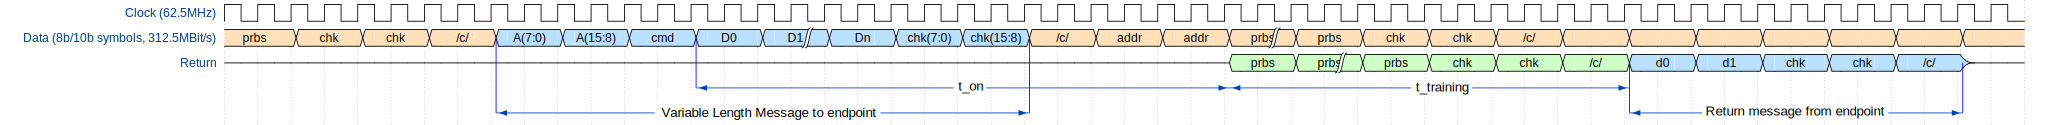
\includegraphics[width=\linewidth]{dts_sp-variable-length-message_ed.pdf}
	\caption{Example timing data stream for a variable length message. The preceding idle packet (also a variable length message) terminates in a comma (/C/ , K28.5) character. The endpoint returns data to the timing master after a period $t_{\mathrm on}$ needed by the endpoint to activate its transmitter plus $t_{\mathrm training}$ needed by the timing master to lock to the signal.}
	\label{fig:wave-variable-length}
\end{figure}

\begin{figure}[h]
	\centering
	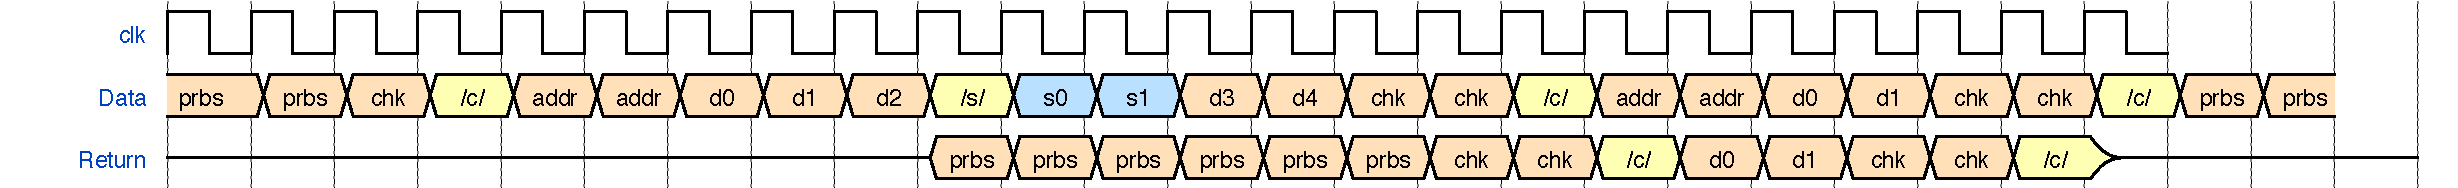
\includegraphics[width=\linewidth]{timing_protocol_wavedrom_01.pdf}
	\caption{Example timing data stream for a variable length message interrupted by a fixed length message. (Fixed length messages have higher priority than variable length).}
	\label{fig:wave-interupted-message}
\end{figure}
\end{landscape}


\subsubsection{Layer 2: Addressing and Protocol}

The synchronous and asynchronous packet formats used in \dword{pdsp2} are shown in Tables~\ref{tab:async}, \ref{tab:sync} and \ref{tab:sync-extra-words}.

\begin{table}[h!]
  \centering
  \begin{tabular}{@{}ll@{}} \toprule
    Byte & Content \\ \midrule
    0 & /S/ (K28.1) \\
    1 & Group / Command \\ \bottomrule
  \end{tabular}
  \caption{Fixed length packet format with no extra words.}
  \label{tab:sync}
\end{table}

\begin{table}[h!]
  \centering
  \begin{tabular}{@{}ll@{}} \toprule
    Byte & Content \\ \midrule
    0 & /S/ (K28.1) \\
    1 & Group / Command \\ 
    2 & word0 \\
    3 & word1 \\
    4 & word2 \\
    5 & word3 \\ 
    6 & word4 \\
    7 & word5 \\
    8 & word6 \\
    9 & word7 \\ 
    \bottomrule
  \end{tabular}
  \caption{Fixed length packet format with four word payload. (For example a timing sync message)}
  \label{tab:sync-extra-words}
\end{table}

\begin{table}[h!]
  \centering
  \begin{tabular}{@{}ll@{}} \toprule
    Byte & Content \\ \midrule
    0 & Address(7:0) \\
    1 & Address(15:8) \\
    2 & Command \\
    3 & Data byte 0 \\ 
    $3 + n$ & Data byte $n$ \\ 
    $3 + n + 1$ & Checksum(7:0) \\
    $3 + n + 2$ & Checksum(15:8) \\
    $3 + n + 3$ & /C/ (K28.5) \\ \bottomrule
  \end{tabular}
  \caption{Variable length packet format}
  \label{tab:async}
\end{table}

Fixed length packets contain a single four-bit timing \dword{group} specifier, and a single four-bit command. Depending on the command type this may be followed by additional words. The number of additional words is determined by the command type. The command field encodes sixteen separate fixed-length commands. Every timing endpoint may be configured with a timing group mask, such that it accept fixed length (synchronous) commands addressed only to selected timing groups. This allows flexible partitioning of the system. Thus there are four independent timing groups and an endpoint can belong to one or more of them.

The timing protocol allows transmission of fixed length commands at a rate of no more than once per 10 clock cycles, which is adequate for the low rate of synchronous commands expected in \dword{pdsp1},\dword{pdsp2} and \dword{dune} \dword{fd}. In the event of clashing fixed length commands, a priority encoding scheme is used, such that lower-numbered commands are transmitted in preference to high-numbered ones, and commands with lower-numbered timing groups are transmitted in preference to commands with higher numbered ones. Under rare or pathological conditions this may result in a fixed length command being rejected; a record is kept of all propagated and rejected signals.

Variable length packets contain a 16-bit address, followed by a single one-byte command followed by an arbitrary number of data bytes. The address is a unique experiment-wide 16b endpoint identifier, or has the special value of 0xfff in the top 12 bits for a broadcast packet, with the timing group identifier in the bottom four bits. The checksum is a standard CRC-16-CCITT, calculated on all packet bytes including the address. Return data packets have identical format. Idle packets are identified by the all-zeroes address, and contain random data which is not interpreted further by the endpoint, except to validate the checksum.

\subsubsubsection{Address Assignment}



%{\color{red}FUTURE\_UPDATE} Document the ProtoDUNE-SP address assignment. Document the ProtoDUNE-SP Run 2 address assignment. Document the DUNE address assignment.

Every active endpoint must have a unique identifier. These are are assigned geographically. Thus, if an endpoint is replaced the replacement hardware must be programmed with the correct address.

\begin{table}[h!]
  \centering
  \begin{tabular}{rll} \toprule
    Field & number of bits & Item \\ \midrule
    C     & 2 & Cavern number (0-1)\\
    S     & 2 & Subsystem 0=TPC,1=PDS,2=Calibration\\
    APA   & 8 & APA number (0-149)\\
    EP    & 4 & Endpoint identifier, e.g. WIB number\\ 
 \bottomrule
  \end{tabular}
  \caption{Components of endpoint address}
  \label{tab:geograpical_addr}
\end{table}

\begin{table}[h!]
  \centering
\begin{bytefield}[endianness=big]{16}
\bitheader{0-15}\\
\bitbox{2}{C} & \bitbox{8}{APA} & \bitbox{2}{S} & \bitbox{4}{EP}
\end{bytefield}
  \caption{Order of bit-fields in endpoint address}
  \label{tab:geograpical_addr_bitfields}
\end{table}



{\color{red}FUTURE\_UPDATE} Define a variable length command that will interrogate a unique ID in the endpoint (c.f. Ethernet MAC address ).

\subsubsubsection{Commands}


The fixed length (synchronous) and variable length (asynchronous) commands currently defined for \dword{pdsp1} and \dword{pdsp2} are shown in Tables~\ref{tab:sync_cmds}, \ref{tab:async_cmds} and \ref{tab:async_ret_cmds}. In the case of fixed-length command queue conflict, priority for transmission is assigned to lower-numbered commands (i.e. counter sync command has priority over all over traffic). Variable length commands meant to be interpreted internally by the timing system endpoint decoder use are distinguished by a 0 in the topmost bit of the command byte.

\begin{table}[h!]
  \centering
  \begin{tabular}{@{}llp{9cm}@{}} \toprule
    Cmd bit & Name & Notes\\ \midrule
    0 & S\_Sync & Used to align and check system cycle counter; issued at 1ms intervals \\
    14 & S\_Spill & SPS spill warning toggle \\
    15 & S\_Trig & Beam trigger signal \\ \bottomrule
  \end{tabular}
  \caption{Fixed length commands}
  \label{tab:sync_cmds}
\end{table}

\begin{table}[h!]
  \centering
  \begin{tabular}{@{}lllp{9cm}@{}} \toprule
    Cmd & Name & Data bytes & Notes\\ \midrule
    0x0 & A\_Reset & 0 & Resets state of endpoint \\
    0x1 & A\_Sync & 8 & Stores cycle counter value to be loaded at next S\_Sync \\
    0x2 & A\_Enable & 0 & Enables endpoint transmission \\
    0x3 & A\_Status & 1 & Request endpoint status packet transmission \\ 
    0x4 & A\_Adjust & 2 & Adjusts packet delay and clock phase of endpoint \\ \bottomrule
  \end{tabular}
  \caption{Variable Length commands}
  \label{tab:async_cmds}
\end{table}

\begin{table}[h!]
  \centering
  \begin{tabular}{@{}lllp{9cm}@{}} \toprule
    Cmd & Name & Data bytes & Notes\\ \midrule
    0x0 & R\_Status & TBD & Endpoint status report \\ \bottomrule
  \end{tabular}
  \caption{Variable length return commands}
  \label{tab:async_ret_cmds}
\end{table}

{\color{red}FUTURE\_UPDATE} Define further fixed length and variable length commands.



\subsubsection{Layer 3: System Level Operations}

The steps required to accomplish basic system level operations are listed below in simplified form. These steps are driven by software inside the timing system which are initiated by the CCM system.

{\color{red}FUTURE\_UPDATE} Add calibration sequences as required.

\subsubsubsection{System Startup}

This procedure is carried out at system startup.

\begin{enumerate}
	\item Reset and initialise timing master unit
	\item Perform master self-test via timing path loopback
	\item Enable command transmission
\end{enumerate}

\subsubsubsection{Phase Adjustment}

This procedure is carried out after endpoints are powered and reset, but before final endpoint initialisation. It is assumed that a 'running' status from the timing decoder will be a necessary step in individual endpoint initialisation sequences. For each endpoint in turn, phase adjustment is carried out as follows:

\begin{enumerate}
	\item The master enables endpoint transmission (by transmitting a A\_Enable command to an endpoint). 
	\item The endpoint responds by starting to transmit idle packets back to the master.
	\item The master waits for CDR lock and measures the clock phase of the signal returning from endpoint
	\item The master sends a status packet request ( A\_Status)
	\item The master measures the number of whole clock cycle in the master $\rightarrow$ endpoint $\rightarrow$ master path. This establishes the delay to / from endpoint
	\item The master issues delay / phase adjustment command ( A\_Adjust ) to the endpoint
	\item The master requests a status packet and verifies correct alignment.
	\item The master sends A\_Disable command to the endpoint and waits until the endpoint has stopped transmitting.
\end{enumerate}

This process is estimated to require around 10ms per endpoint (dominated by the time required for CDR lock and clock phase measurement), allowing \dword{pdsp2} to be brought up in a few seconds.

{\color{red}FUTURE\_UPDATE} Document measured phase adjustment time as measured in hardware.

\subsubsubsection{Operations Startup}

This procedure is carried out after all endpoints are aligned, and after time-of-day is established via GPS.

\begin{enumerate}
	\item Reset master cycle counter
	\item Enable command and input logging
	\item Enable regular S\_Sync commands
	\item Enable trigger commands
\end{enumerate}

\subsubsubsection{System Monitoring}

System monitoring is continually carried out by continuous repetition of the endpoint phase check sequence, and logging of any error counts reported by endpoints. This activity has lower priority than other system activities.

\subsubsubsection{Operations Shutdown}

This procedure is carried out after all DAQ queues have drained, as one of the last end-of-run steps.

\begin{enumerate} 
	\item Disable trigger commands
	\item Wait until next S\_Sync command
	\item Disable regular S\_Sync commands
	\item Issue S\_Reset
	\item Disable command and input logging
\end{enumerate}




\clearpage

\printglossary
\printbibliography

\end{document}
 